\documentclass[12pt]{article}

\usepackage{cite}
\usepackage{amsmath,amssymb,amsfonts}
\usepackage{algorithmic}
\usepackage{graphicx}
\usepackage{textcomp}
\usepackage{xcolor}
\usepackage{float}
\usepackage{subfigure}
\usepackage{listings}
\usepackage{color}
\usepackage{geometry}
\geometry{a4paper,left=3.5cm,right=3.5cm,top=2.5cm,bottom=2.5cm}

\definecolor{dkgreen}{rgb}{0,0.6,0}
\definecolor{gray}{rgb}{0.5,0.5,0.5}
\definecolor{mauve}{rgb}{0.58,0,0.82}

\lstset{frame=tb,
  language=Python,
  aboveskip=3mm,
  belowskip=3mm,
  showstringspaces=false,
  columns=flexible,
  basicstyle={\small\ttfamily},
  numbers=none,
  numberstyle=\tiny\color{gray},
  keywordstyle=\color{blue},
  commentstyle=\color{dkgreen},
  stringstyle=\color{mauve},
  breaklines=true,
  breakatwhitespace=true,
  tabsize=3
}

\begin{document}

\title{\textbf{Gesture Recognition Based On Deep Learning}}
\author{Runlin Hou \and Sifan Yuan \and Yuxiang Song \and Haocong Wang}
\maketitle

\section{Introduction}
\section{Dataset}
\section{Model}
\section{Implementaion}
In this section, we are going to talk about how we implement the network and training process. We seperatet this section into three parts according to the code, which corresponding to implement the models, resizing of the dataset, and the whole training process.
\subsection{Model Implementation}
For our project, we implement two classic CNN models, which are LeNet5 and ResNet34. As we mentioned above, LeNet5 is a simple CNN model with 7 layers, which is relatively small compared to ResNet34. And of course, a smaller size of the model always corresponding to a relatively poorer performance. With a larger scale, ResNet34 can deal with more parameters and consequently results in a better capability to a larger scale image. And we will show a more detailed test result in the next section.
\subsubsection*{LeNet5}
There is only 7 layers (exclusion of the input layer) in the LeNet5, so we can easily implement layer by layer with Pytorch. In section 3 we mentioned that LeNet5 is consist of convolutional layers and fully connected layers, which all have their packged function in Pytorch. 

But for our project something we need to pay attention to is that the input channel of the first convolutional layer. Since we have two dataset to train on and one of them is an RGB dataset, but the original LeNet5 is designed for gray scale image, we need to make the LeNet5 enable to deal with the 3-channel RGB images. Therefore, we adjust the input channel according to the input dataset. Also, the dataset does not share same amount of classes included, which means the final output also needed to be matched with dataset.

\begin{lstlisting}
  class LeNet5(nn.Module):
    def __init__(self, class_num, is_gray_scale):
        super(LeNet5, self).__init__()

        if is_gray_scale:
            input_channel = 1
        else:
            input_channel = 3

    ......

    def num_flat_features(self, x):
        size = x.size()[1:]
        num_features = 1
        for s in size:
            num_features *= s
        return num_features
\end{lstlisting}

\subsubsection*{ResNet34}
Since ResNet34 got a much more complex structure compared to LeNet5 and includes a repetive structure called residual block, we will implement the residual block first to simplify the code. As we mentioned in section 3, a classic residual block always consist of two convolutional layers with batchnorm process between. Also, in the forward computing process, the key of residual network is to add $x$ to the layer output $H(x)$ to get $H(x)+x$ to compute the residual. Following the typically methods, we implement this residual block.
\begin{lstlisting}
  class ResBlock(nn.Module):
    def __init__(self, inchannel, outchannel, stride=1, shortcut=None):
        super(ResBlock, self).__init__()
        self.basic = nn.Sequential(
            nn.Conv2d(inchannel, outchannel, 3, stride, 1, bias=False),
            nn.BatchNorm2d(outchannel),
            nn.ReLU(inplace=True),
            nn.Conv2d(outchannel, outchannel, 3, 1, 1, bias=False),
            nn.BatchNorm2d(outchannel),
        )
        self.shortcut = shortcut

    def forward(self, x):
        out = self.basic(x)
        residual = x if self.shortcut is None else self.shortcut(x)
        out += residual
        return nn.ReLU(inplace=True)(out)
\end{lstlisting}

After we got the residual block class, we can construct the whole network by the superposition of multiple residual blocks. In our project we choose to implement a 34-layer residual network. Before the residual learning process, we first have a convolutional layer for the normalize of the input images to make them fit the subsequent residual block layers. Then we have 4 groups of residual block layers. The first layer have 3 residual blocks with 64 input channels and 128 output channels. The second layer has 4 residual blocks with 128 input channels and 256 output channels. The third layer has 6 residual block with 256 input channels and 512 output channels. The fourth layer has 3 residual blcok with 512 input channels and 512 output channels. Then the network end up with a fully connected layer for the prediction result. So the network has 1 initial convolutional layer and 32 convolutional layers in residual block and one last fully connected layer for output prediction, which are 34 layers in total.

Similarly with LeNet5, our project requires the network to fit the two datasets we have. Also, we want to test how the model work on the gray scale images compared to RGB images. To achieve this requirement, we have the input channel of the first convolutional layer and the output of the last fully connected layer to be adjustable. 

\begin{lstlisting}
  class ResNet34(nn.Module):
    def __init__(self, class_num, is_gray_scale):
        super(ResNet34, self).__init__()
        if is_gray_scale:
            input_channel = 1
        else:
            input_channel = 3

        self.pre = nn.Sequential(
            nn.Conv2d(input_channel, 64, 7, 2, 3, bias=False),
            nn.BatchNorm2d(64),
            nn.ReLU(inplace=True),
            nn.MaxPool2d(3, 2, 1),)
        self.layer1 = self.__make_layer__(64, 128, 3)
        self.layer2 = self.__make_layer__(128, 256, 4, stride=2)
        self.layer3 = self.__make_layer__(256, 512, 6, stride=2)
        self.layer4 = self.__make_layer__(512, 512, 3, stride=2)
        self.fc = nn.Linear(512, class_num)
        ......

    def forward(self, x):
        ......

        return self.fc(x)
\end{lstlisting}

\subsection{Datasets Adjustment}
In our project, we have two datasets for training as we mentioned in section 2. The first one is sign language mnist dataset, the amount of this dataset are huge compared to the kinect leap dataset. Since this dataset is actually designed for the LeNet, the size of images inside the dataset is $28\times 28$, which is relatively small compared to the other one. This make us a problem that the images are too small for the ResNet34, the images are unacceptable for ResNet34 since the images are smaller than a convolutional core of the first convolutional layre. Meanwhile, LeNet5 can neither learning an image with too large scale. So the main purpose of this part is to deal with the size of the input images. Considering all the requirements mentioned above, we choose to resize the image to $224 \times 224$ for ResNet34 and $28\times 28$ for LeNet5.

Also, another factor we want to experiment on is that he whether the gray scale of the the image influenced the training result. To fullfill this purpose we add a trigger to the dataset dealing process, which allow us to choose to output the images in 1 channel our 3 channels. 

\begin{lstlisting}
  class dataset_loader:
    ......

    def load_sign_mnist(self, img_size, isGrayScale):
        ......

    def load_kinect_leap(self, img_size, isGrayScale, train_size=1200):
        all_data = self.load_kinect_leap_dataset()
        shuffle(all_data)

        # set train and test set
        train_data = all_data[0:train_size - 1]
        train_set = KinectLeapDataset(train_data, img_size=img_size, is_gray_scale=isGrayScale)
        train_loader = DataLoader(dataset=train_set, batch_size=8, shuffle=False)

        test_data = all_data[train_size:len(all_data) - 1]
        test_set = KinectLeapDataset(test_data, img_size=img_size, is_gray_scale=isGrayScale)
        test_loader = DataLoader(dataset=test_set, batch_size=8, shuffle=False)

        return train_loader, test_loader

    def load_kinect_leap_dataset(self):
        ......
    
  class KinectLeapDataset(Dataset):
    def __init__(self, data, img_size, is_gray_scale=False):
        print('loading kinect_leap_dataset')

        self.data = data
        self.labels = []
        self.is_gray_scale = is_gray_scale
        for label_tp in self.data:
            self.labels.append(label_tp[0])

        self.height = img_size
        self.width = img_size
        self.transform = transforms.Compose([transforms.ToTensor()])

    def __getitem__(self, index):
        single_image_label = self.labels[index]
        img_as_np = np.asarray(self.data[index][1])
        img_as_img = Image.fromarray(img_as_np)

        img_as_img = img_as_img.resize((self.height, self.width))

        if self.is_gray_scale:
            img_as_img = img_as_img.convert('L')

        if self.transform is not None:
            img_as_tensor = self.transform(img_as_img)

        return (img_as_tensor, single_image_label)

    def __len__(self):
        return len(self.data)
\end{lstlisting}

Here we take \verb|KinectLeapDataset| as an example, resizing process of the image is embeded in the \verb|.__getitem__()| function for each Pytorch \verb|dataset| class. Later by \verb|DataLoader()| class, we convert the dataset into certain size iterable batches of images in \verb|Tensor| format.

\subsection{Traing Process}
With all tools we needed, which are models and datasets. The training process are quite simple to build. For thr criterion and optimizer we choose to use \verb|CorssEntropyLoss| and \verb|SGD| optimizer. 

Also, we use a tool package \verb|tensorboardX| to monitor the training process, whose result is going to be shown in the next section.

\section{Test Result}
In this sectoin, we are going to talk about the result of the training process. We totally run six different settings to find out how the performance can be influenced by input dataset, gray scale of the images and network itself.

\begin{figure}[H]
    \centering

    \subfigure[Le-MNIST-gray]{
        \begin{minipage}[b]{0.3\textwidth}
            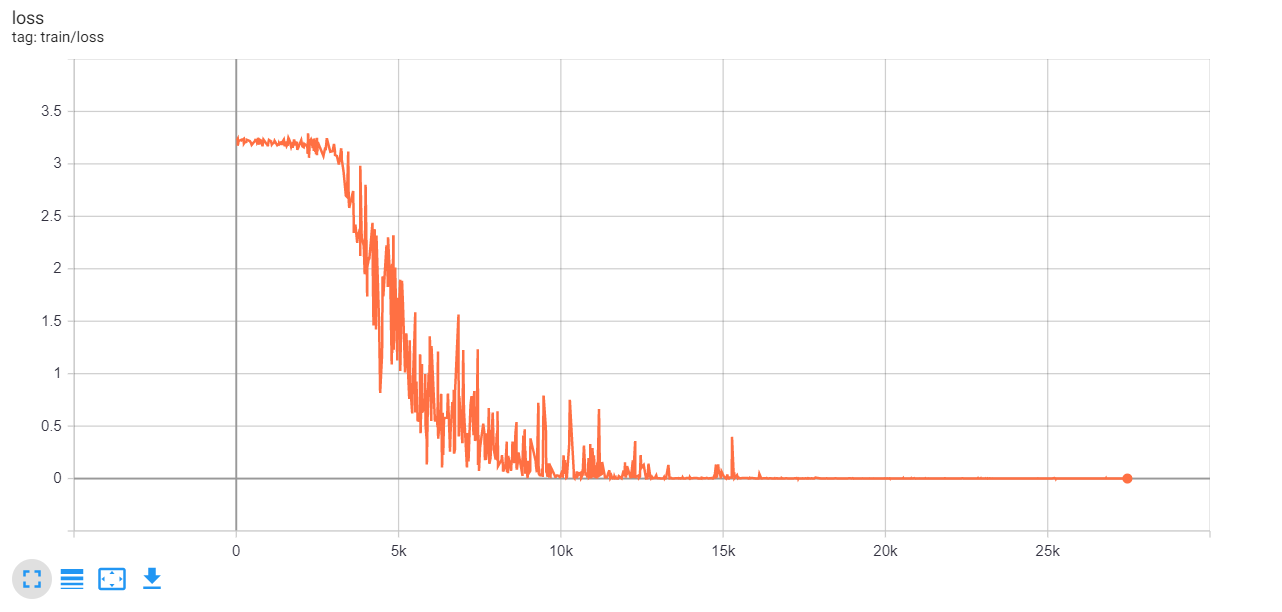
\includegraphics[width=1.1\textwidth]{pic/LeNet5GraymnistLoss.png}
        \end{minipage}
    }
    \subfigure[Le-leap-gray]{
        \begin{minipage}[b]{0.3\textwidth}
            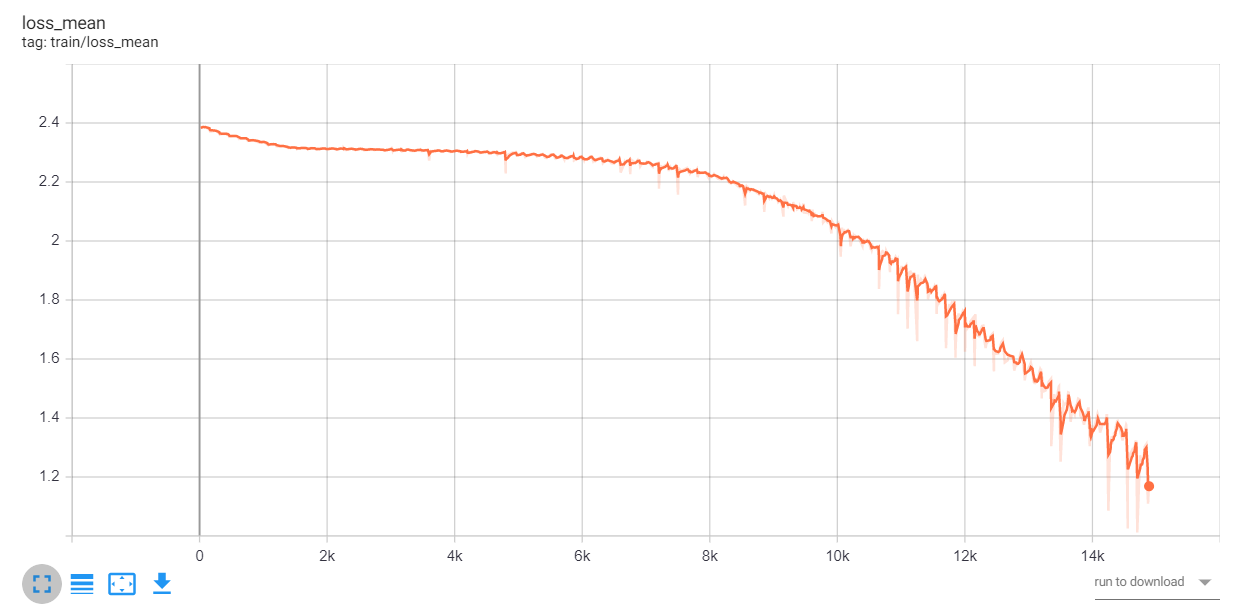
\includegraphics[width=1.1\textwidth]{pic/LeNet5grayleaploss.png}
        \end{minipage}
    }
    \subfigure[Le-leap-RGB]{
        \begin{minipage}[b]{0.3\textwidth}
            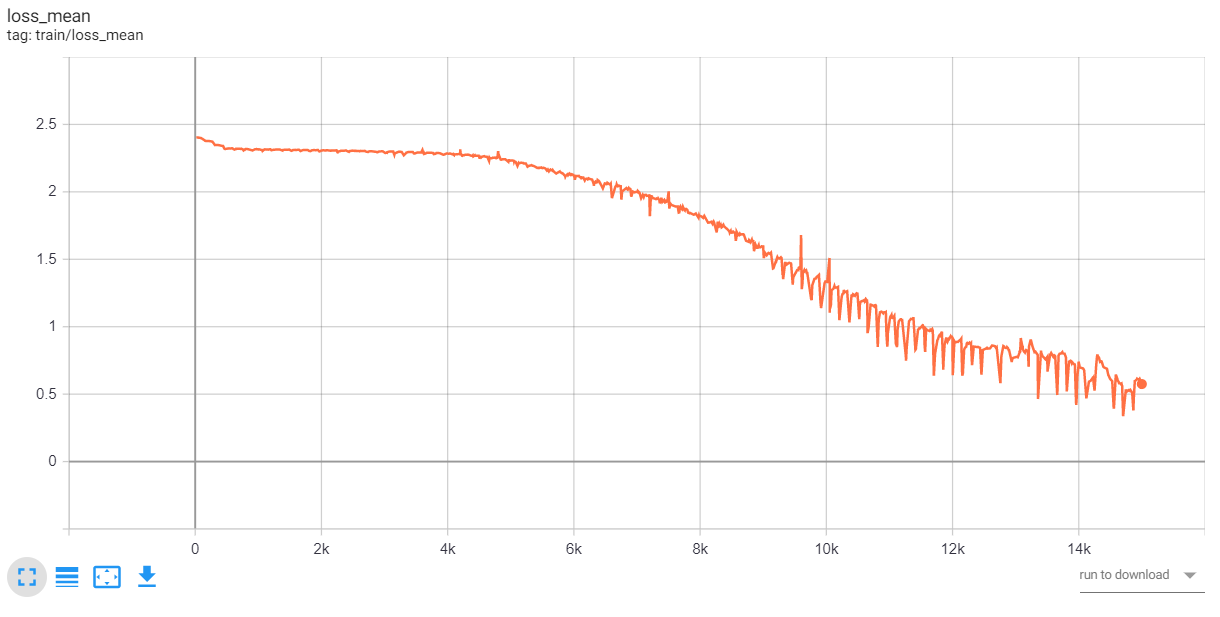
\includegraphics[width=1.\textwidth]{pic/LeNet5leaprgbloss.png}
        \end{minipage}
    }
    \\
    \subfigure[Res-MNIST-gray]{
        \begin{minipage}[b]{0.3\textwidth}
            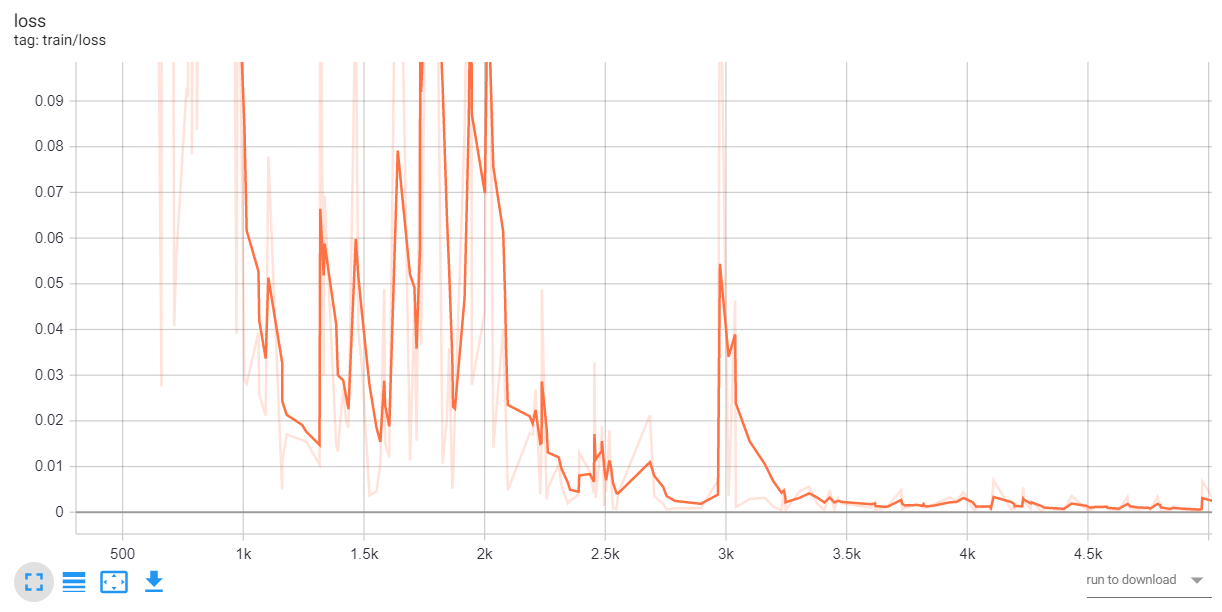
\includegraphics[width=1.1\textwidth]{pic/ResNetmnistloss.png}
        \end{minipage}
    }
    \subfigure[Res-leap-gray]{
        \begin{minipage}[b]{0.3\textwidth}
            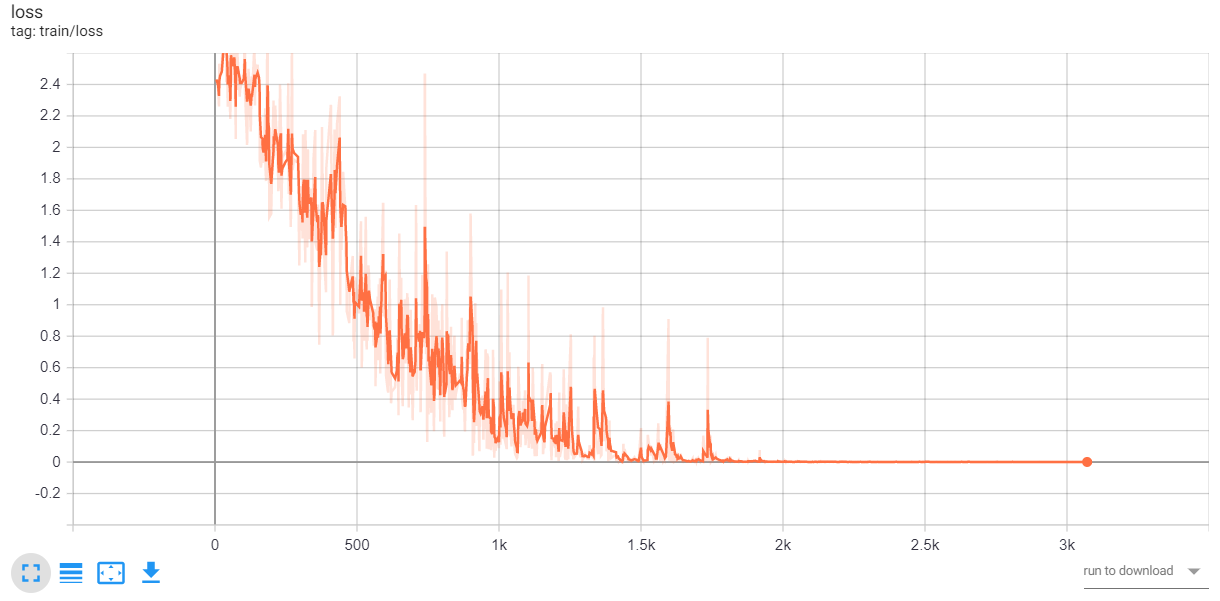
\includegraphics[width=1.1\textwidth]{pic/ResNetleaploss.png}
        \end{minipage}
    }
    \subfigure[Res-leap-RGB]{
        \begin{minipage}[b]{0.3\textwidth}
            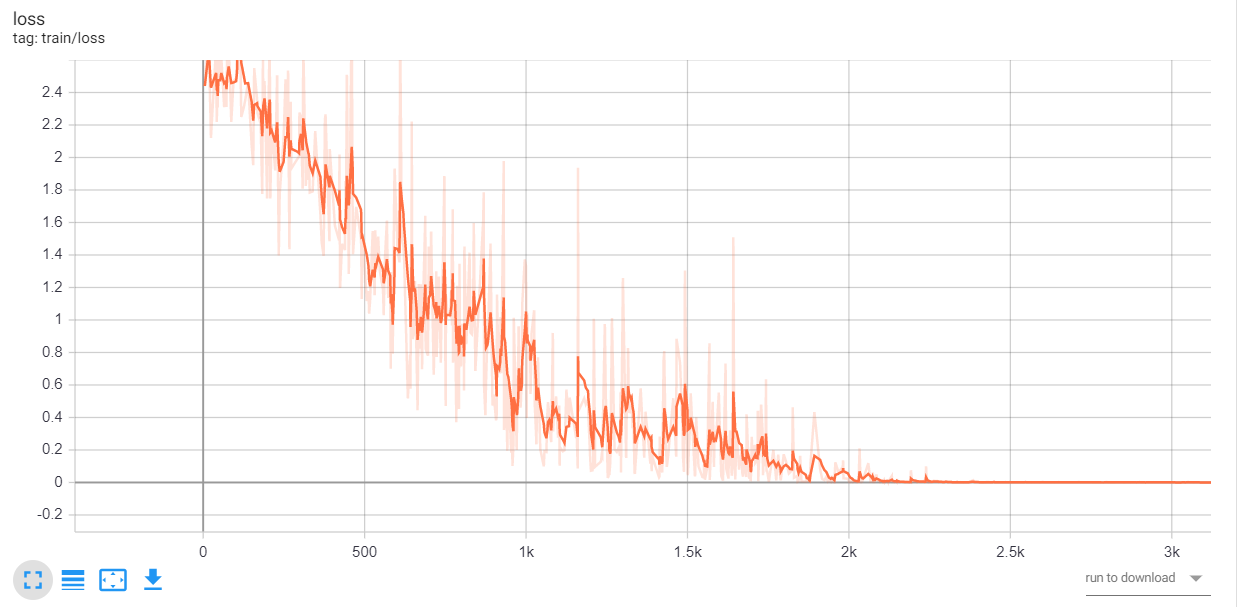
\includegraphics[width=1.1\textwidth]{pic/ResNetleaprgbloss.png}
        \end{minipage}
    }


    \caption{Variation of the loss during the training process.}
\end{figure}


\begin{figure}[H]
    \centering

    \subfigure[Le-MNIST-gray]{
        \begin{minipage}[b]{0.3\textwidth}
            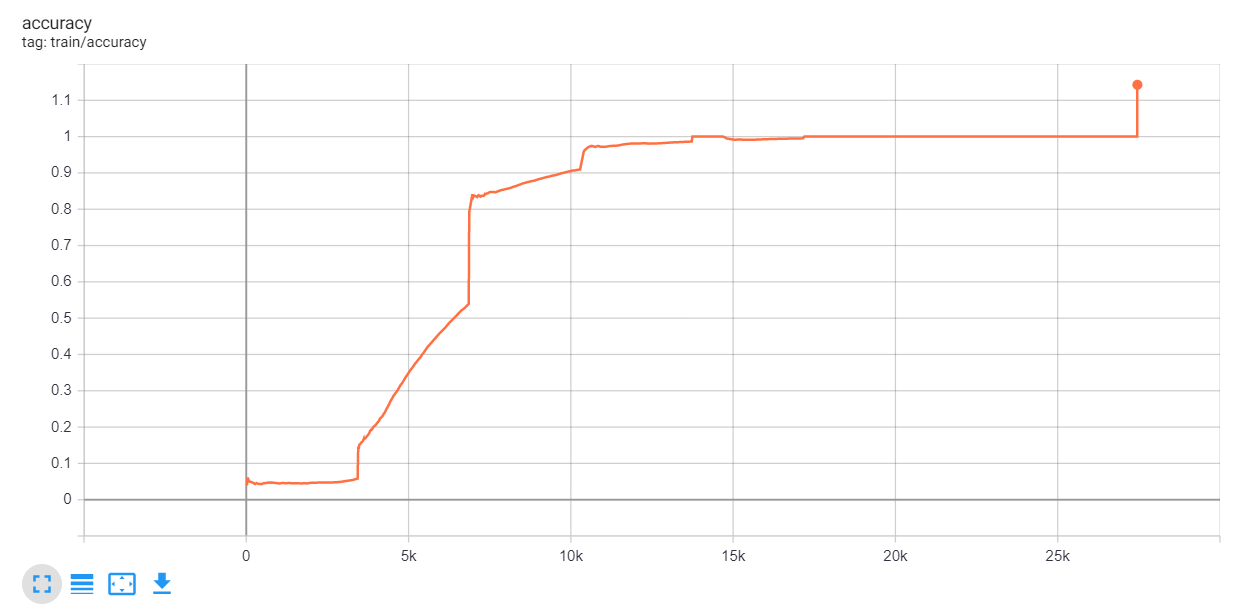
\includegraphics[width=1.1\textwidth]{pic/LeNet5Graymnist.png}
        \end{minipage}
    }
    \subfigure[Le-leap-gray]{
        \begin{minipage}[b]{0.3\textwidth}
            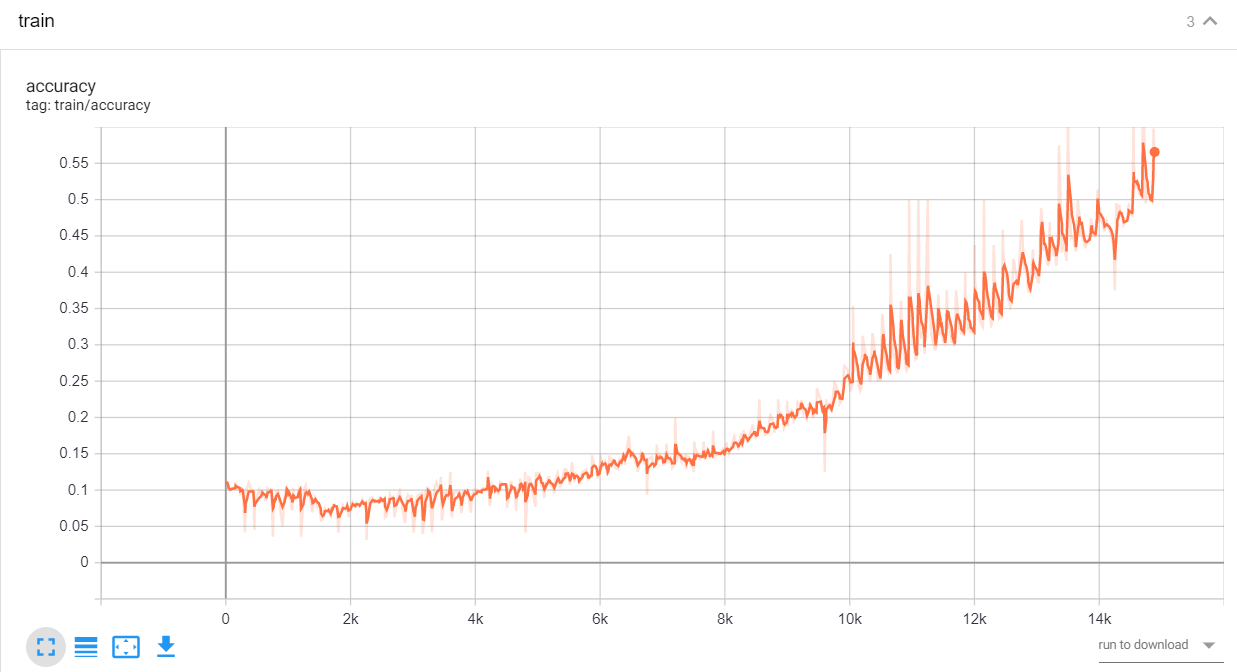
\includegraphics[width=1.1\textwidth]{pic/LeNet5grayleaptrain.png}
        \end{minipage}
    }
    \subfigure[Le-leap-RGB]{
        \begin{minipage}[b]{0.3\textwidth}
            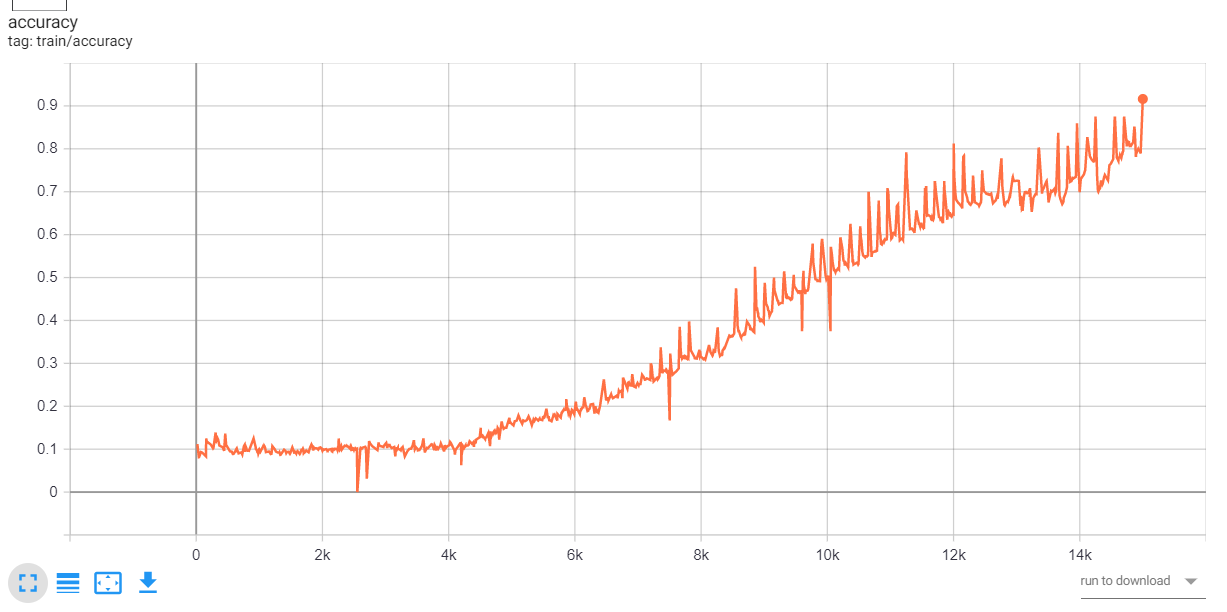
\includegraphics[width=1.\textwidth]{pic/LeNet5leaprgbtrain.png}
        \end{minipage}
    }
    \\
    \subfigure[Res-MNIST-gray]{
        \begin{minipage}[b]{0.3\textwidth}
            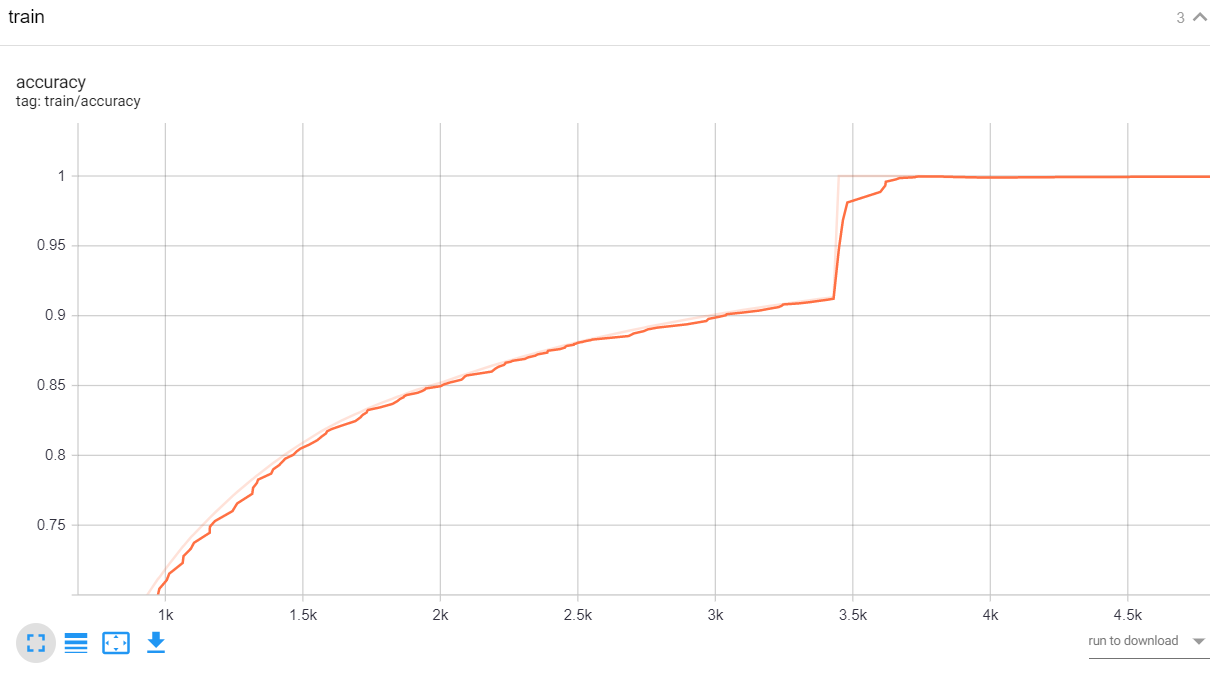
\includegraphics[width=1.1\textwidth]{pic/ResNetmnisttrain.png}
        \end{minipage}
    }
    \subfigure[Res-leap-gray]{
        \begin{minipage}[b]{0.3\textwidth}
            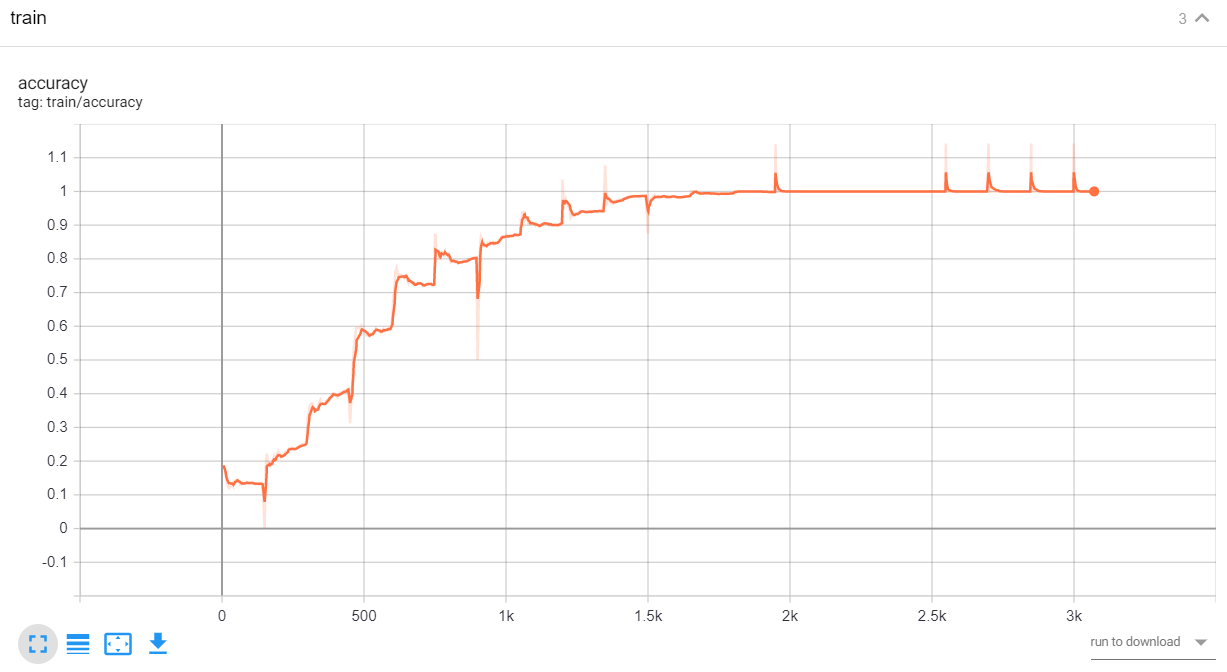
\includegraphics[width=1.1\textwidth]{pic/ResNetleaptrain.png}
        \end{minipage}
    }
    \subfigure[Res-leap-RGB]{
        \begin{minipage}[b]{0.3\textwidth}
            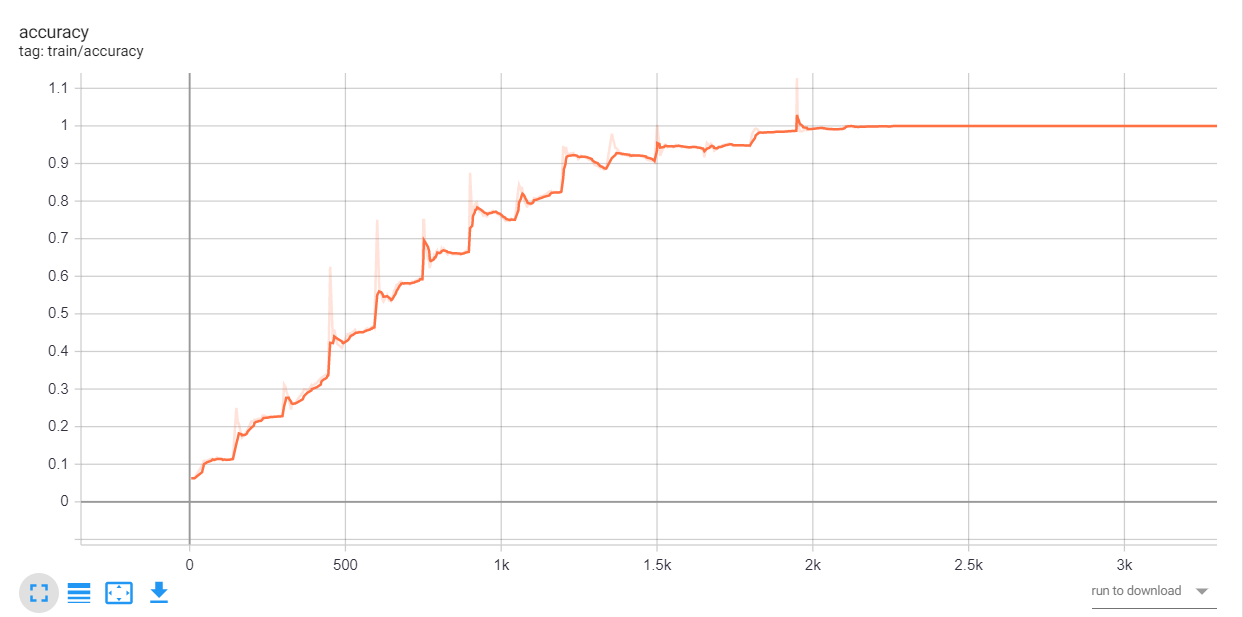
\includegraphics[width=1.1\textwidth]{pic/ResNetleaprgbtrain.png}
        \end{minipage}
    }


    \caption{Variation of the accuracy during the training process.}
\end{figure}

\begin{figure}[H]
    \centering

    \subfigure[Le-MNIST-gray]{
        \begin{minipage}[b]{0.3\textwidth}
            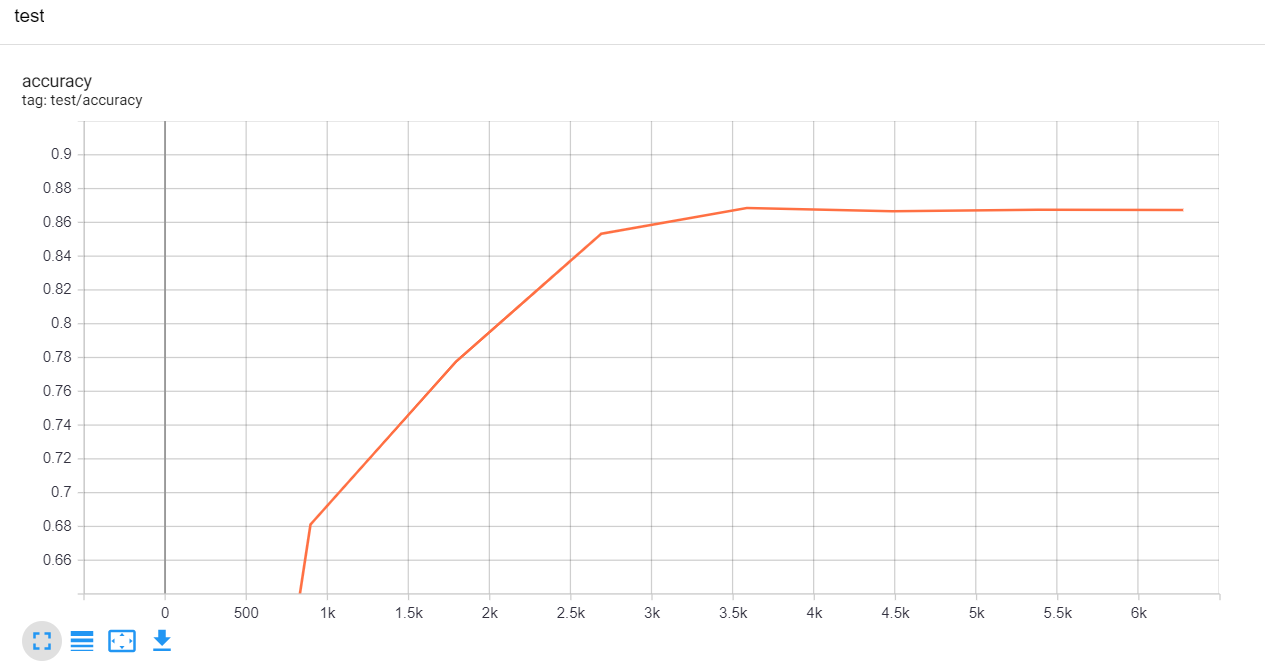
\includegraphics[width=1.1\textwidth]{pic/LeNet5GraymnistTest.png}
        \end{minipage}
    }
    \subfigure[Le-leap-gray]{
        \begin{minipage}[b]{0.3\textwidth}
            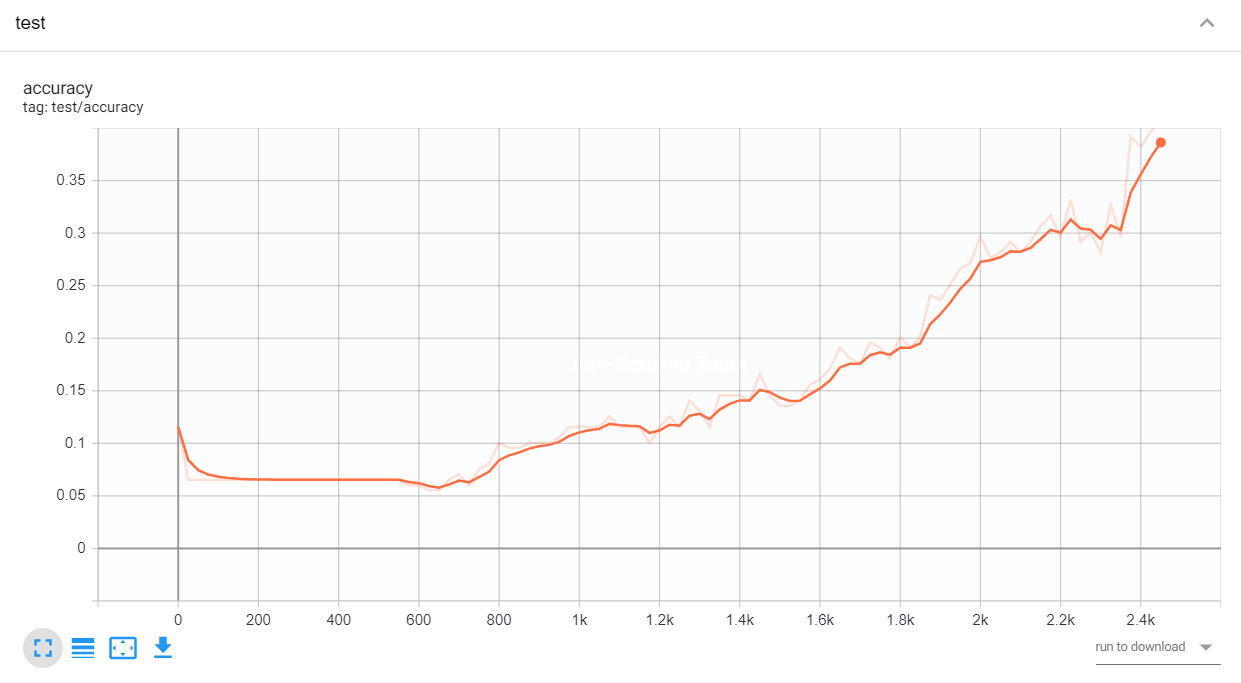
\includegraphics[width=1.1\textwidth]{pic/LeNet5grayleaptest.png}
        \end{minipage}
    }
    \subfigure[Le-leap-RGB]{
        \begin{minipage}[b]{0.3\textwidth}
            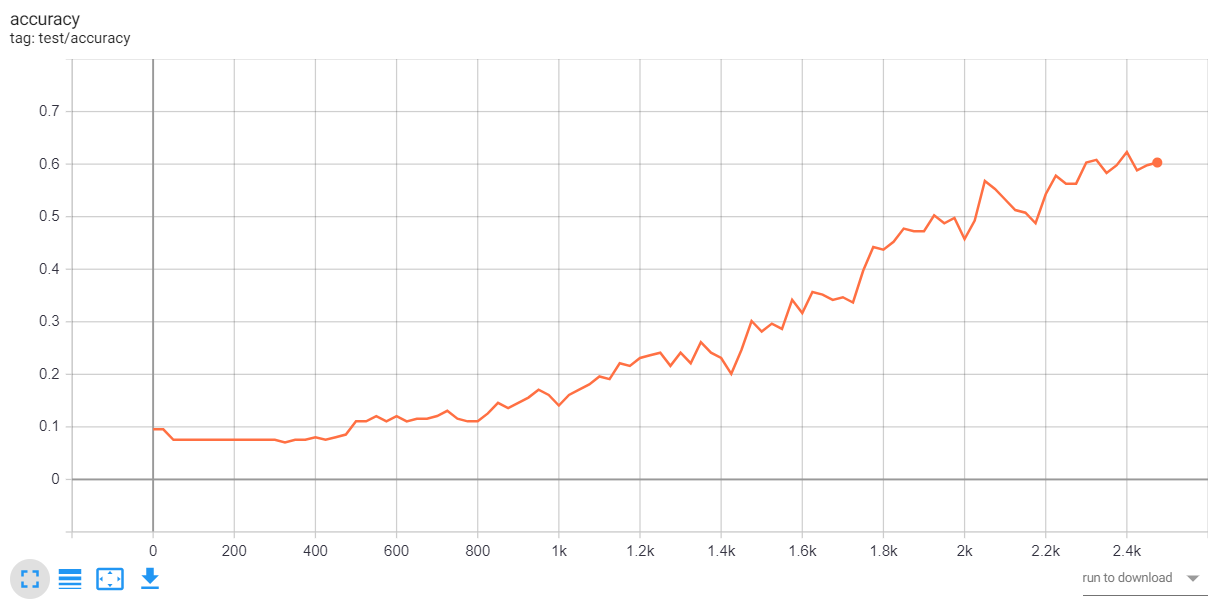
\includegraphics[width=1.\textwidth]{pic/LeNet5leaprgbtest.png}
        \end{minipage}
    }
    \\
    \subfigure[Res-MNIST-gray]{
        \begin{minipage}[b]{0.3\textwidth}
            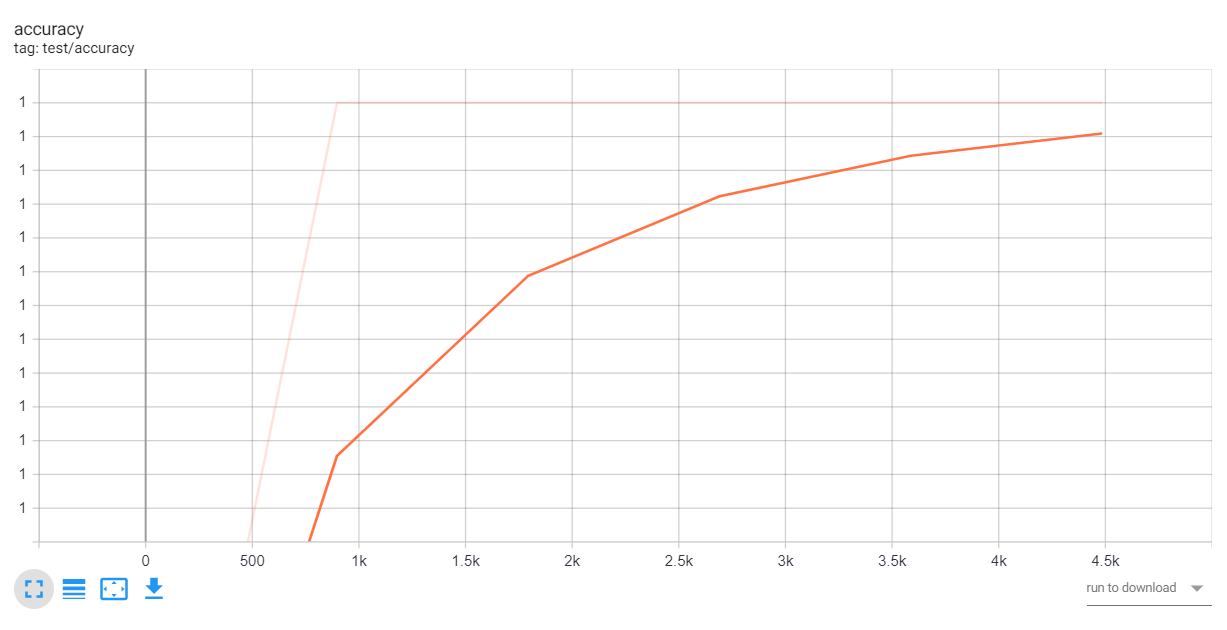
\includegraphics[width=1.1\textwidth]{pic/ResNetmnisttest.png}
        \end{minipage}
    }
    \subfigure[Res-leap-gray]{
        \begin{minipage}[b]{0.3\textwidth}
            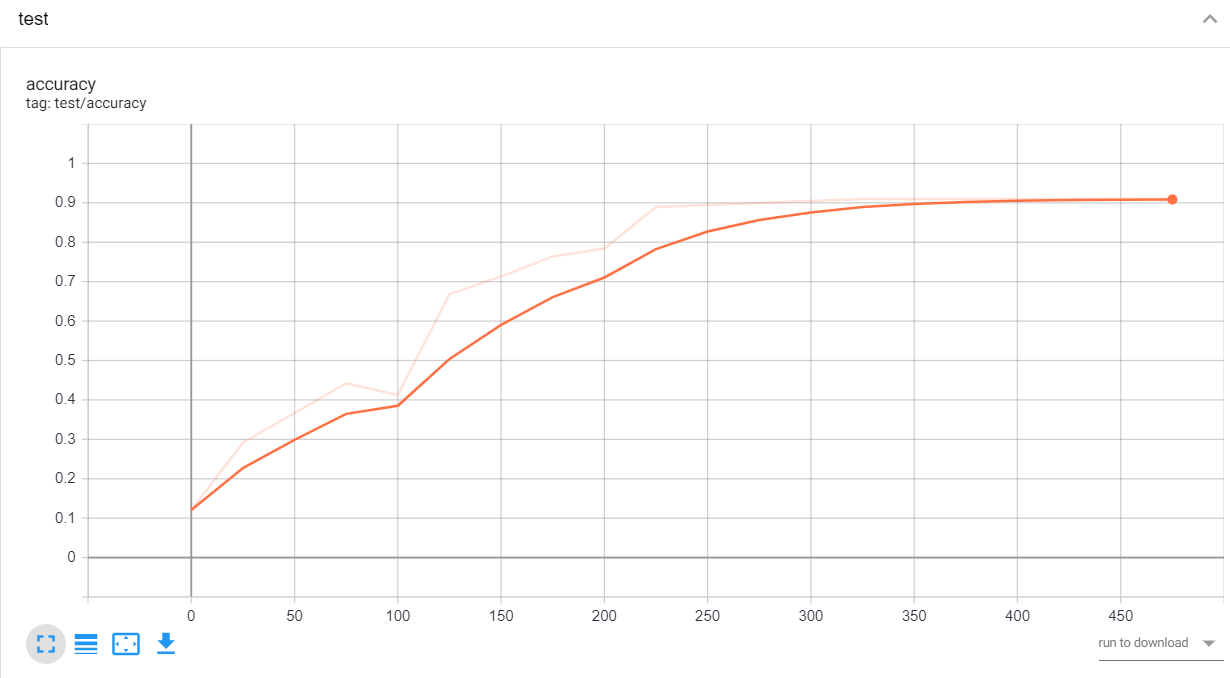
\includegraphics[width=1.1\textwidth]{pic/ResNetleaptest.png}
        \end{minipage}
    }
    \subfigure[Res-leap-RGB]{
        \begin{minipage}[b]{0.3\textwidth}
            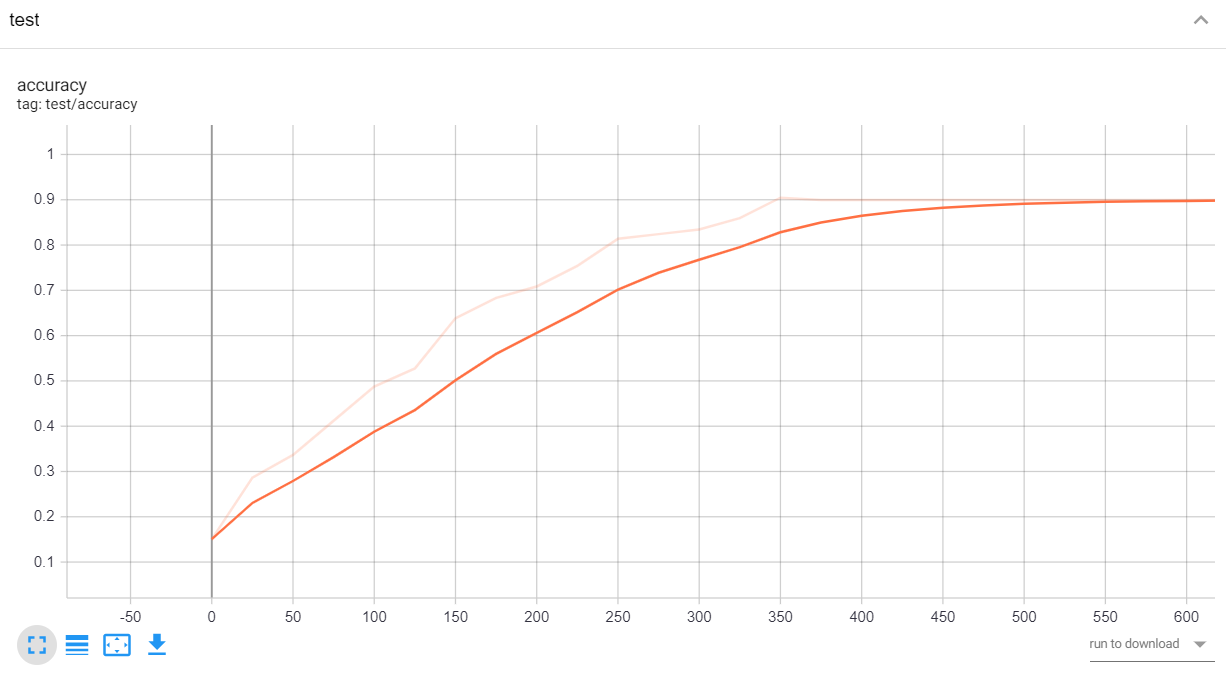
\includegraphics[width=1.1\textwidth]{pic/ResNetleaprgbtest.png}
        \end{minipage}
    }


    \caption{Variation of the accuracy during the testing process.}
\end{figure}

As we can see in the above, the first group of charts shows how the loss variate in the training process with different settings. For LeNet5, there is a clearly slowdown on the speed of the loss reduction. pic(a) shows that when dealing with the MNIST dataset, LeNet5 can reduce the loss to almost zero within 15k images. But for kinect leap dataset with larger scale of images, LeNet5 can not do so well. When the amount of fed images comes to 15k, the loss only reduced to around 1.2, which is actually an unacceptable performance. The result is getting a little better when we change the images into RGB format, loss can fall around 0.5. 

Respectively, the accuracy performances under each settings are highly corresponding to the loss reduction. So, imaginablely, accuracy when LeNet5 dealing with the MNIST dataset is actually pretty well that can reach 100\% in training process and 87\% in testing process. But when it came to kinect leap dataset, the even the training accuracy can only reach 55\% and the testing accuracy is no more than 40\%. The RGB images setting basicly shares the same result. 

The performance of ResNet34 shows much better performance on both datasets. On sign language mnist dataset, loss can be reduced to almost zero around 3.5k. When facing the kinect leap dataset, ResNet34 surprisingly did even better than on MNIST dataset. Loss reaches almost 0 before 2k. For RGB images ResNet34 take 0.5k more images to reach the same level.

The result are also pretty well for accuracy. In the training process, all accuracy can reach 100\%. And for test process ResNet34 can also reach 90\% accuracy which is relatively higher than the performance of LeNet5.

In conclusion, we can say that there is no doubt that ResNet34 shows a better performance. And for gray scale, this attribute has raletively low affect on the final result. Since every gray scale image is actually generate from an RGB image, we can say that each gray scale image mentains enough information from gray sacle images. LeNet5 shows poor performance compared to ResNet34, espacially on the large scale image. But one of its advantages is that the small scale of this network, which leads to a smaller computational resource.

\section{Application}
\section{Future Work \& Conclusion}

\end{document}


